\newcommand{\icol}[1]{% inline column vector
  \left(\begin{smallmatrix}#1\end{smallmatrix}\right)%
}

\newcommand{\irow}[1]{% inline row vector
  \begin{smallmatrix}(#1)\end{smallmatrix}%
}
\chapter{Optimization of OpenStreetMap Building Footprints~Based on Semantic Information of Oblique UAV Images}
%: Querying and Understanding EO Archives}
\label{ch:lucas_arch}

OpenStreetMap (OSM) is a collaborative project for creating a free editable map of the world based on volunteered geographic information. It is able to provide free and updated geographic information despite restrictions on usage or availability of georeferenced data across most of the world. In recent years, OSM has widely expanded its coverage and gained increasing popularity in many applications. One~example is the generation of 3D building models from OSM building footprints \cite{Goetz2012towards}. Therefore, the quality of building reconstruction and modeling strongly relies on the quality of building footprints. A~detailed analysis for OSM building footprints \cite{fan2014quality} assessed a high completeness accuracy and a position accuracy of about 4 m on average for these data. Therefore, OSM building footprints can be safely regarded as a rough approximation of the real scene.

Though numerous approaches for building footprint generation have been developed, most~of them exploit information from airborne imagery \cite{mueller2005robust} or point cloud data \cite{zhou20102}, where the building footprints are represented by roofs and therefore usually mixed with overhangs. In contrast, building fa\c{c}ades naturally contain critical information about footprints. In this sense, data that presents fa\c{c}ade information, such as oblique airborne imagery and terrestrial point clouds, can facilitate accurate building footprints' generation. Among different data sources, oblique UAV 
%Define if appropriate
imagery stands out as it bridges the gap between aerial and terrestrial mapping, thus enabling data acquisition of both building roofs and fa\c{c}ades simultaneously. 


Given an initial hypothesis of the building boundary, the refinement with well-designed constraints plays a vital role in improving the accuracy of building footprints. The constraints usually come from the 3D features embedded in DSMs 
%Define if appropriate
or point clouds as well as from the 2D features in images. For the case of oblique UAV images, 3D features such as lines \cite{lafarge2012creat} and planes usually have low geometric accuracy due to the change of the viewing directions in oblique images \cite{xiao2015building}. Apart from that, image features can also be employed as effective constraints. Traditional methods employed color features \cite{Sirmacek2008building} in early stages, which are vulnerable to shadows and illumination. Some methods extracted building boundaries by detecting 2D lines \cite{zhu2015feature} or corners \cite{wegner2009fusion}. However, the detected edges or corners have uncertain semantic meanings and therefore can only be used as weak evidence. In contrast, pixel-wise semantic image segmentation provides an effective solution to this problem. Various handcrafted features have been proposed in traditional machine learning based classification tasks. For instance, 2D image features, 2.5D~topographic features and 3D geometric features are integrated in \cite{gevaert2017informal} for supervised classification using an~SVM classifier. With the rapid development of deep neural networks, deep-learning based segmentation methods have demonstrated their conspicuous advantages in yielding reliable and robust semantic segmentation compared to traditional machine-learning segmentation methods. Deconvolution networks are firstly applied in \cite{huang2016building} for building extraction from remote sensing images and demonstrate promising segmentation accuracy.

In this paper, we aim to refine the building footprint in OSM by deploying textural features from multi-view images as constraints. Based on the above discussion on previous research, we are motivated to use oblique UAV images as data sources for footprint generation. Constraints for solving the optimization problem are defined by building boundaries, i.e., the projection of the 3D building model on images, are expected to lie on the boundary between building fa\c{c}ades and the ground. The~contour evidence is extracted from pixel-wise semantic segmentation via deep convolution neural networks. The proposed method is composed of these steps: first, we geo-register the UAV images by matching them with high-accuracy aerial images; meanwhile, we perform semantic segmentation of UAV images using a Fully Convolutional Network (FCN) and extract the boundaries between building fa\c{c}ades, roof and ground as contour evidence; then, we initialize a 3D building model of LoD 1 
%Define if appropriate
from the OSM footprints, followed by an optimization that integrates the contour evidence of multi-view images as a constraint. In the end, not only the footprints, but also the building heights get optimized. The proposed method is tested on different datasets. The accuracy of the optimized OSM footprints is evaluated by comparison with the ATKIS 
%Define if appropriate
data, whose position accuracy is around 0.5 m \cite{muller1998quality}. 


The main innovations of this paper lie in the following aspects:
\begin{itemize}
\item The footprints addressed in previous research are the roof areas with overhangs. In contrast, our~method is able to detect the real building footprints excluding roof overhangs, i.e., the~edges where the building fa\c{c}ades meet the ground.
\item Instead of directly detecting buildings in 3D space, we introduce an optimization scheme using the image evidence from pixel-wise segmentation as a constraint, i.e., the image projection of the building model is encouraged to be identical to the building areas detected via pixel-wise image~segmentation. 
\item Our method is able to refine simultaneously the building footprint and its height.  
\end{itemize}


The paper is organized as follows: Section \ref{sec:related} gives a brief literature review on building footprint generation and points out the drawbacks of state-of-the-art methods regarding this topic. Section \ref{sec:method} describes our approach for OSM footprint optimization in detail. In Section \ref{sec:exp}, experiments on various datasets are carried out to validate the feasibility and robustness of the proposed method. Furthermore, the accuracy of the optimized building footprints is evaluated both qualitatively and quantitatively by comparing with the ATKIS data. Finally, Section \ref{sec:conclu} discusses potentials and limitations of the proposed method and describes further applications.

\section{Related Work}\label{sec:related}
Obtaining accurate building footprints is of paramount importance in many applications such as urban planning or the real estate industry. Many attempts have been made to automatic ally extract building footprints in the last few decades. Traditionally, satellite imagery, aerial imagery and LiDAR data are among the most widely used data sources in this context. Some of the studies exploit solely information from images via pixel-based or object-based segmentation. Various segmentation descriptors \cite{DORNAIKA2016130} have been developed and other image features such as shadows \cite{ok2013exploiting} are also used for this purpose. Nevertheless, it is usually difficult to extract accurate building outlines from only images due to occlusion, shades and low illumination. Therefore, some studies explore the geometric features embedded in 3D data, e.g., Digital Surface Model (DSM) \cite{dini2013delineation}, point cloud reconstructed from images \cite{dai2017building} and LiDAR data \cite{awrangjeb2014automatic}, or integrate the information from imagery and 3D data together \cite{bittner2017building, li2013fusion}. However, these approaches are also prone to occlusions and have difficulties in detecting precise building boundaries. Moreover, as the building fa\c{c}ades are inherently hardly visible in nadir-view remote sensing data, the aforementioned approaches actually extract building roofs rather than the real footprint without overhangs.

Considering that building fa\c{c}ades convey vital information on building footprints, the data containing fa\c{c}ade information, such as terrestrial data or oblique airborne imagery, can facilitate building footprint generation. A building detection method based on oblique aerial images is proposed in \cite{nex2013building}, while the fa\c{c}ade information in terrestrial LiDAR point cloud is exploited \cite{Hammoudi2009ExtractingBF, yang2013semiautomated}. As a bridge between terrestrial and airborne photogrammetry, the UAV stands out for its ability to achieve high spatial and temporal resolutions compared to traditional remote sensing platforms. Additionally, it~has a great advantage in the application of building footprint generation for its ability in delivering information on both building roofs and fa\c{c}ades. The accuracy of 3D building modeling based on both nadir and oblique UAV images is studied in \cite{vacca2017the}, demonstrating that the integration of oblique UAV images can substantially increase the achievable accuracy comparing to traditional modeling using the terrestrial point cloud.




 



% \section{Analysis}\label{sec:analy}
% \subsection{quality assessment of OSM building footprints}
% The accuracy of building footprints is usually measured in three aspects, namely, completeness, position accuracy and shape accuracy. Figure \ref{fig:osm_error} illustrates the errors of building footprints in OSM.
% \begin{figure}[H]
%     \centering
%        \begin{subfigure}[tbp]{0.32\columnwidth}
%            \centering
%            \includegraphics[width=\textwidth]{analysis/incomplete.png}
%            \caption[]{completeness}
%            {{\small }}
%            \label{fig:com}
%        \end{subfigure}
%        \hfill
%        \begin{subfigure}[tbp]{0.32\columnwidth}
%            \centering
%            \includegraphics[width=\textwidth]{analysis/shift1.png}
%            \caption[]{position}%
%            {{\small }}
%            \label{fig:shift}
%        \end{subfigure}
%        \hfill
%        \begin{subfigure}[tbp]{0.32\columnwidth}
%            \centering
%            \includegraphics[width=\textwidth]{analysis/shift2.png}
%            \caption[]{shape}%
%            {{\small }}
%            \label{fig:shape}
%        \end{subfigure}
%        \caption{}
%        \label{fig:osm_error}
% \end{figure}

% \subsection{extracting buildings from UAV point cloud}
% Though the point cloud is generated using the well-known commercial software Pix4D, the reconstructed UAV point cloud still suffer from occlusion and low overlap, resulting in low-quality point cloud where most building fa\c{c}ades are missing, as shown in Figure \ref{fig:pc_hole}. 
% \begin{figure}[H]
%     \centering
%        \begin{subfigure}[tbp]{0.5\columnwidth}
%            \centering
%            \includegraphics[width=\textwidth]{analysis/pc_hole.png}
%            \caption[]{}
%            {{\small }}
           
%        \end{subfigure}
%        \caption{point cloud reconstructed from oblique UAV images}
%        \label{fig:pc_hole}
% \end{figure}

\section{Methodology}\label{sec:method}
In this section, we give a detailed account of the proposed approach for optimization of the OSM building footprint. The proposed workflow is comprised of the following steps: (1) geo-registration of oblique-view UAV images; (2) semantic segmentation of UAV images using a Fully Convolutional Network (FCN); and (3) optimization of the building model initialized from OSM footprints. We also point out the conditions and restrictions for the proposed method. Figure \ref{fig:flow} depicts the workflow of the proposed approach. The external input data includes the building footprint extracted from OSM and the DSM reconstructed from aerial images, from which we can initialize a simple building sketch. In parallel, we create a ground truth dataset of UAV images and fine-tune the FCN-8s model. The~trained network is then applied to segment UAV images. Finally, we optimize the building sketch by minimizing the chamfer distance between the building outline from projection and the contour evidence from image segmentation. Details of each step are explained in the following paragraphs. 

\begin{figure}[H]
    \centering       
           \centering
           \includegraphics[width=\textwidth]{method/flowchart.png} 
       \caption{Workflow of the proposed method. External input data includes the building footprint extracted from OSM and DSM 
%Define if appropriate       
reconstructed from aerial images, from which a building sketch is initialized. Meanwhile, we create a ground truth dataset and fine-tune the FCN-8s 
%Define if appropriate
model for image segmentation. We optimize the building sketch by minimizing the chamfer distance between the building outline from projection and the contour evidence from image segmentation.}
       \label{fig:flow}
\end{figure}


\subsection{Geo-Registration of UAV Images}
The geo-registration of UAV images has already been discussed in numerous research works. One~of the biggest challenges lies in the automated orientation of oblique UAV images. Towards this goal, various solutions have been proposed. Commercial softwares (e.g., Pix4D, Agisoft) and open source softwares (e.g., Bundler,  PMVS,  VisualSFM,  MicMac) are widely used for matching and structure from motion (SFM) of oblique-view UAV images \cite{lingua20173d,aicardi2016UAV}. An image pyramid-based stratified matching method for matching nadir and oblique images from four-combined cameras in the step of structure from motion is proposed in \cite{xie2012study}, while an AKAZE 
%Define if appropriate
interest operator-based matching strategy is presented in \cite{onyango2017accurate} for automatic registration of oblique UAV imagery to oblique aerial imagery.

Another challenge is the accurate geo-registration of UAV image blocks. Although UAV images are usually coupled with on-board GNSS/INS information, their absolute
%Define if appropriate
accuracy, solely 3 to 5 m in cases without a correction signal, is no higher than the one of OSM building footprints. In contrast, the accuracy of aerial photogrammetry can achieve a $10^{-2}$ m level, which notably exceeds OSM and is sufficient for our application. We adopt the approach proposed in \cite{zhuo2017automatic} for co-registration between low-accuracy UAV images and high-accuracy aerial images. In short, the method assumes that the aerial images are geo-referenced and have common overlap with UAV images. First, the camera poses of sequential UAV images are solved via Structure From Motion (SFM), and then the nadir UAV images with the aerial images are matched using the proposed matching scheme and generate thousands of reliable image correspondences. Given accurate camera poses of the aerial images, the 3D coordinates of those common image correspondences can be calculated via image-to-ground projection. These 3D points are then adopted to estimate the camera poses of the corresponding nadir-view UAV images. In the end, those UAV images with known camera poses are involved in a global optimization for camera poses of all UAV images. In this way, all UAV images are co-registered to the aerial images. The absolute accuracy of the geo-registered UAV images, according to the paper, can be as good as a $10^{-1}$ m level.

The aforementioned approach requires georeferenced aerial images of the surveyed area. In the absence of such reference images, the UAV images can be geo-registered with manually established \hl{Ground Control Points (GCPs)}, %capitalized
which may come from \hl{RTK GPS} surveys 
%Define if appropriate
or measurements from geo-spatial products (e.g., Basemap) with higher accuracy. For example, we can create some \hl{GCPs} %already defined 
by measuring their planar coordinates $(x,y)$ on an orthophoto and their elevation values $z$ on a DSM. The GCPs with coordinates $(x,y,z)$ can then be deployed to geo-register the UAV images dataset. 

\subsection{Semantic Segmentation of UAV Images}
Extracting building outlines in images is essentially an issue of object recognition. Meanwhile, building outlines can also be viewed as class boundaries, which can be obtained from pixel-wise semantic segmentation. In this sense, the semantic segmentation of UAV images plays a crucial role in our pipeline as our optimization relies on the building outlines extracted from the segmentation as the constraint. Considering the fact that deep learning based methods significantly outperform traditional machine learning methods using handcrafted features, we attempt to train a deep neural network for the task of semantic segmentation.

Typically, a Convolutional Neural Network (CNN) is composed of an input layer, an output layer and multiple hidden layers in between. The hidden layers generally include convolutional layers, pooling layers, fully connected layers and normalization layers. In particular, convolutional layers apply nonlinear operations on the input with a set of adjustable parameters, which can be learned during the training process. The results are then passed to the next layer. Pooling layers take the outputs of neuron blocks of one layer and subsample them into a single neuron. A CNN may contain several convolutional layers and pooling layers. All the neurons in previous layers are then connected by a fully connected layer to each individual neuron in another layer. In order to adapt the classifier for a dense prediction, a solution has to consider these fully connected layers as convolutions with kernels covering their entire input regions \cite{fcn}. Compared to the evaluation of the original classification network on overlapping input patches, the adapted classifier, namely FCN, is more efficient since computational burdens are shared by overlapping regions of patches. The network used in this paper is a modification of \cite{fcn} by changing the number of outputs according to our demand. In~our experiment, there are seven classes in total, i.e., building, roof, ground, road, vegetation, vehicle and clutter. The architecture of the neural network is depicted in Figure \ref{fig:archi}.

The aforementioned FCN also has shortcomings. First, its receptive field is as large as 32 pixels, resulting in segments with non-sharp boundaries and blob-like shapes. However, sharp boundaries between buildings and surroundings are preferred for us. Second, the prediction of FCN does not take the smoothness and the consistency of label assignments into consideration. To solve this problem, we plug in a Conditional Random Field (CRF) represented as Recurrent Neural Network (CRFasRNN) \cite{crfasrnn_ICCV2015,higherordercrf_ECCV2016} at the end of the FCN, which combines the strengths of both the CNN and CRF based graphical model in one unified framework. In this model, unary energies are obtained from the FCN, which~predict labels of pixel without considering the smoothness and the consistency of the label assignments; meanwhile, the pairwise energies provide a data-dependent smoothing term that encourages semantic label coherence for pixels with similar properties. Such combination enhances the consistency of the changes in labeling and in image intensity, resulting in sharp boundaries between adjacent segments.

For the compensation of limited training data, we implement data augmentation by cropping, rotating and scaling. Instead of training the network from scratch, we initialize the network with pre-trained weights from the FCN-8s model and then fine-tune it with our own ground-truth data. Details of implementation and parameter settings are described in Section \ref{sec:exp}. 

In the end, we deploy the trained network to generate pixel-wise semantic segmentations of the images. Since the building footprint is defined as the boundary of a building where it meets the ground, the edge model of building footprints, denoted by $L_0$, can be therefore extracted as the boundary between the class ``building'' and the class ``ground'' from the semantically labeled images. It needs to be pointed out that semantic segmentation itself does not have a concept of an object; however, we are interested in class boundaries, which can be seen as objects that should be detected.


\begin{figure}[H]
    \centering
       \begin{subfigure}[tbp]{0.9\columnwidth}
           \centering
           \includegraphics[width=\textwidth]{method/structure.png}
           
                    
       \end{subfigure}
       \caption{Architecture of the FCN network used in this paper.}
       \label{fig:archi}
\end{figure}



\subsection{Optimization of Building Footprints}

We consider the building model as a polyhedron in 3D space featured by the building footprint $\mathscr{P}$ and height $H$. In particular, $\mathscr{P}$ is comprised of a set of vertices $\{ P_{1},  \ldots ,  P_{n} \mid  P_{i} \subset \mathbb{R}^3 \}$, where $P_{i}$ denotes the 3D coordinates $\icol{X_{i}\\Y_{i}\\Z_{i}}$ of each corner of the building footprint, which can be directly extracted from OSM. For the cases without OSM height information, we can obtain the elevation of the ground at the foot of the building as well as the elevation of the roof, denoted by $Z_{ground}$ and $Z_{roof}$, respectively, in~a~DSM from aerial imagery using a Top-Hat transform algorithm \cite{shih2009image,Mongus2012tophat}. Then, the elevation $Z_{ground}$ is assigned to $Z_{i}$ and the difference \hl{$Z_{roof} - Z_{ground}$} is assigned to the building height $H$. At this point, a~simple building model formulated by footprint and a uniform height has been established.

% Consider the building footprint as a polygon in 3D space: $\mathscr{P} \subset \mathbb{R}^3$ with vertices $\left [ \icol{X_{1}\\Y_{1}\\Z}, \ldots , \icol{X_{n}\\Y_{n}\\Z} \right]$ arranged in clockwise order. Where, $\irow{X_{i}&Y_{i}}$ denotes the planar coordinates of each bottom corner of the building, which can be directly extracted from OSM; $Z$ denotes the elevation of the footprint, which can be roughly estimated with the help of the Google Earth or a DSM of this area.
%


With geo-registered UAV images, the corresponding image point projection of $\mathscr{P}$ can be simply computed by means of ground-to-image projection, resulting in a 2D polygon denoted by $\mathscr{S}$ $\subset$ $\mathbb{R}^2$. 
% with vertices $\left [ \icol{x_{1}\\y_{1}} , ... , \icol{y_{n}\\y_{n}} \right]$. 
Theoretically, if $\mathscr{P}$ is absolutely accurate, its projection $\mathscr{S}$ should be exactly identical with the building area in the UAV image. Under the assumption that the image segmentation result is reliable, the~edge model of the polygon $\mathscr{S}$, denoted by $L_1$, should be close to the edge model $L_0$ extracted from the segmented image. Hereby, we adopt the Chamfer Distance \cite{BORGEFORS1986distance} as a measurement for the difference between $L_0$ and $L_1$. We first cut off the area of $L_0$ from the image with a buffer zone of 100 pixels as the region of interest (ROI), and then generate the distance image of $L_0$. Afterwards, we superimpose $L_1$ on the distance image and the Chamfer Distance between $L_0$ and $L_1$ is defined as:
\begin{equation} \label{eq:1}
D(L_0,L_1) = \sqrt{\frac{1}{N} \sum_{l\in L_1}^{} d_{I(l)}^2},
\end{equation}
where $d_{I(l)}$ stands for the distance values where the edge model $L_1$ hits the distance image of $L_0$, while~\emph{N} is the number of points in $L_1$. 

One building may be present in multiple images from different viewing directions, and these images may have different segmentation accuracy in building areas. Despite the high interior accuracy of the images' block, the image derived building contours in different images have a certain degree of variance, resulting in different Chamfer Distance. Therefore, it makes sense to take all cases into consideration. The adjustment of OSM footprints can be formulated as an energy minimization problem whose energy term is defined as Equation (\ref{eq:2}). In particular, $\mathscr{I}$ denotes the set of images that show the building, vector $P_{i}$ denotes each vertex in the OSM footprint to be optimized, while $H$ stands for the height of the building:

\begin{equation} \label{eq:2}
\begin{split}
 \underset{x}{\text{minimize}}  
& \quad E = \sum_{i\in \mathscr{I}^{}} D(L_{0}^{(x, i)}, D(L_{1}^{(x, i)}),\\
& x = \{\{ P_{1},  \ldots ,  P_{n}, H \mid  P_{i} \subset \mathbb{R}^3, H \in \mathbb{R}  \}\}.
\end{split}
\end{equation}

We solve the minimization problem using a modification of Powell’s method \cite{powell1964efficient, press1989numerical}, which performs sequential one-dimensional minimizations along each vector of the directions set. After optimization, the~accuracy of the building footprint and height improves. 





\subsection{Application Conditions}
It should be pointed out that building footprints can only be partially optimized in the presence of occlusions. Figure \ref{fig:3a} shows the projection of an original OSM footprint in an aerial image, while Figure \ref{fig:3b} highlights the edges that can be optimized with the proposed method. Figure \ref{fig:3c} is an aerial image of the surveyed area with a slightly oblique view. Given that no additional images are available, only the visible building borders (marked with red lines) can be optimized. Towards the goal to achieve a complete optimization of the building footprints, it is thereby advised to acquire UAV images of the buildings of interest from different viewing directions so that all the fa\c{c}ades are visible in the images.

 

\begin{figure}[H]
    \centering
       \begin{subfigure}[tbp]{0.43\columnwidth}
           \centering
           
           \includegraphics[width=\textwidth]{analysis/proj_3k.png}
           \caption[]{}
           {{\small }} 
           \label{fig:3a}
       \end{subfigure}
       \hfill
       \begin{subfigure}[tbp]{0.4\columnwidth}
           \centering
           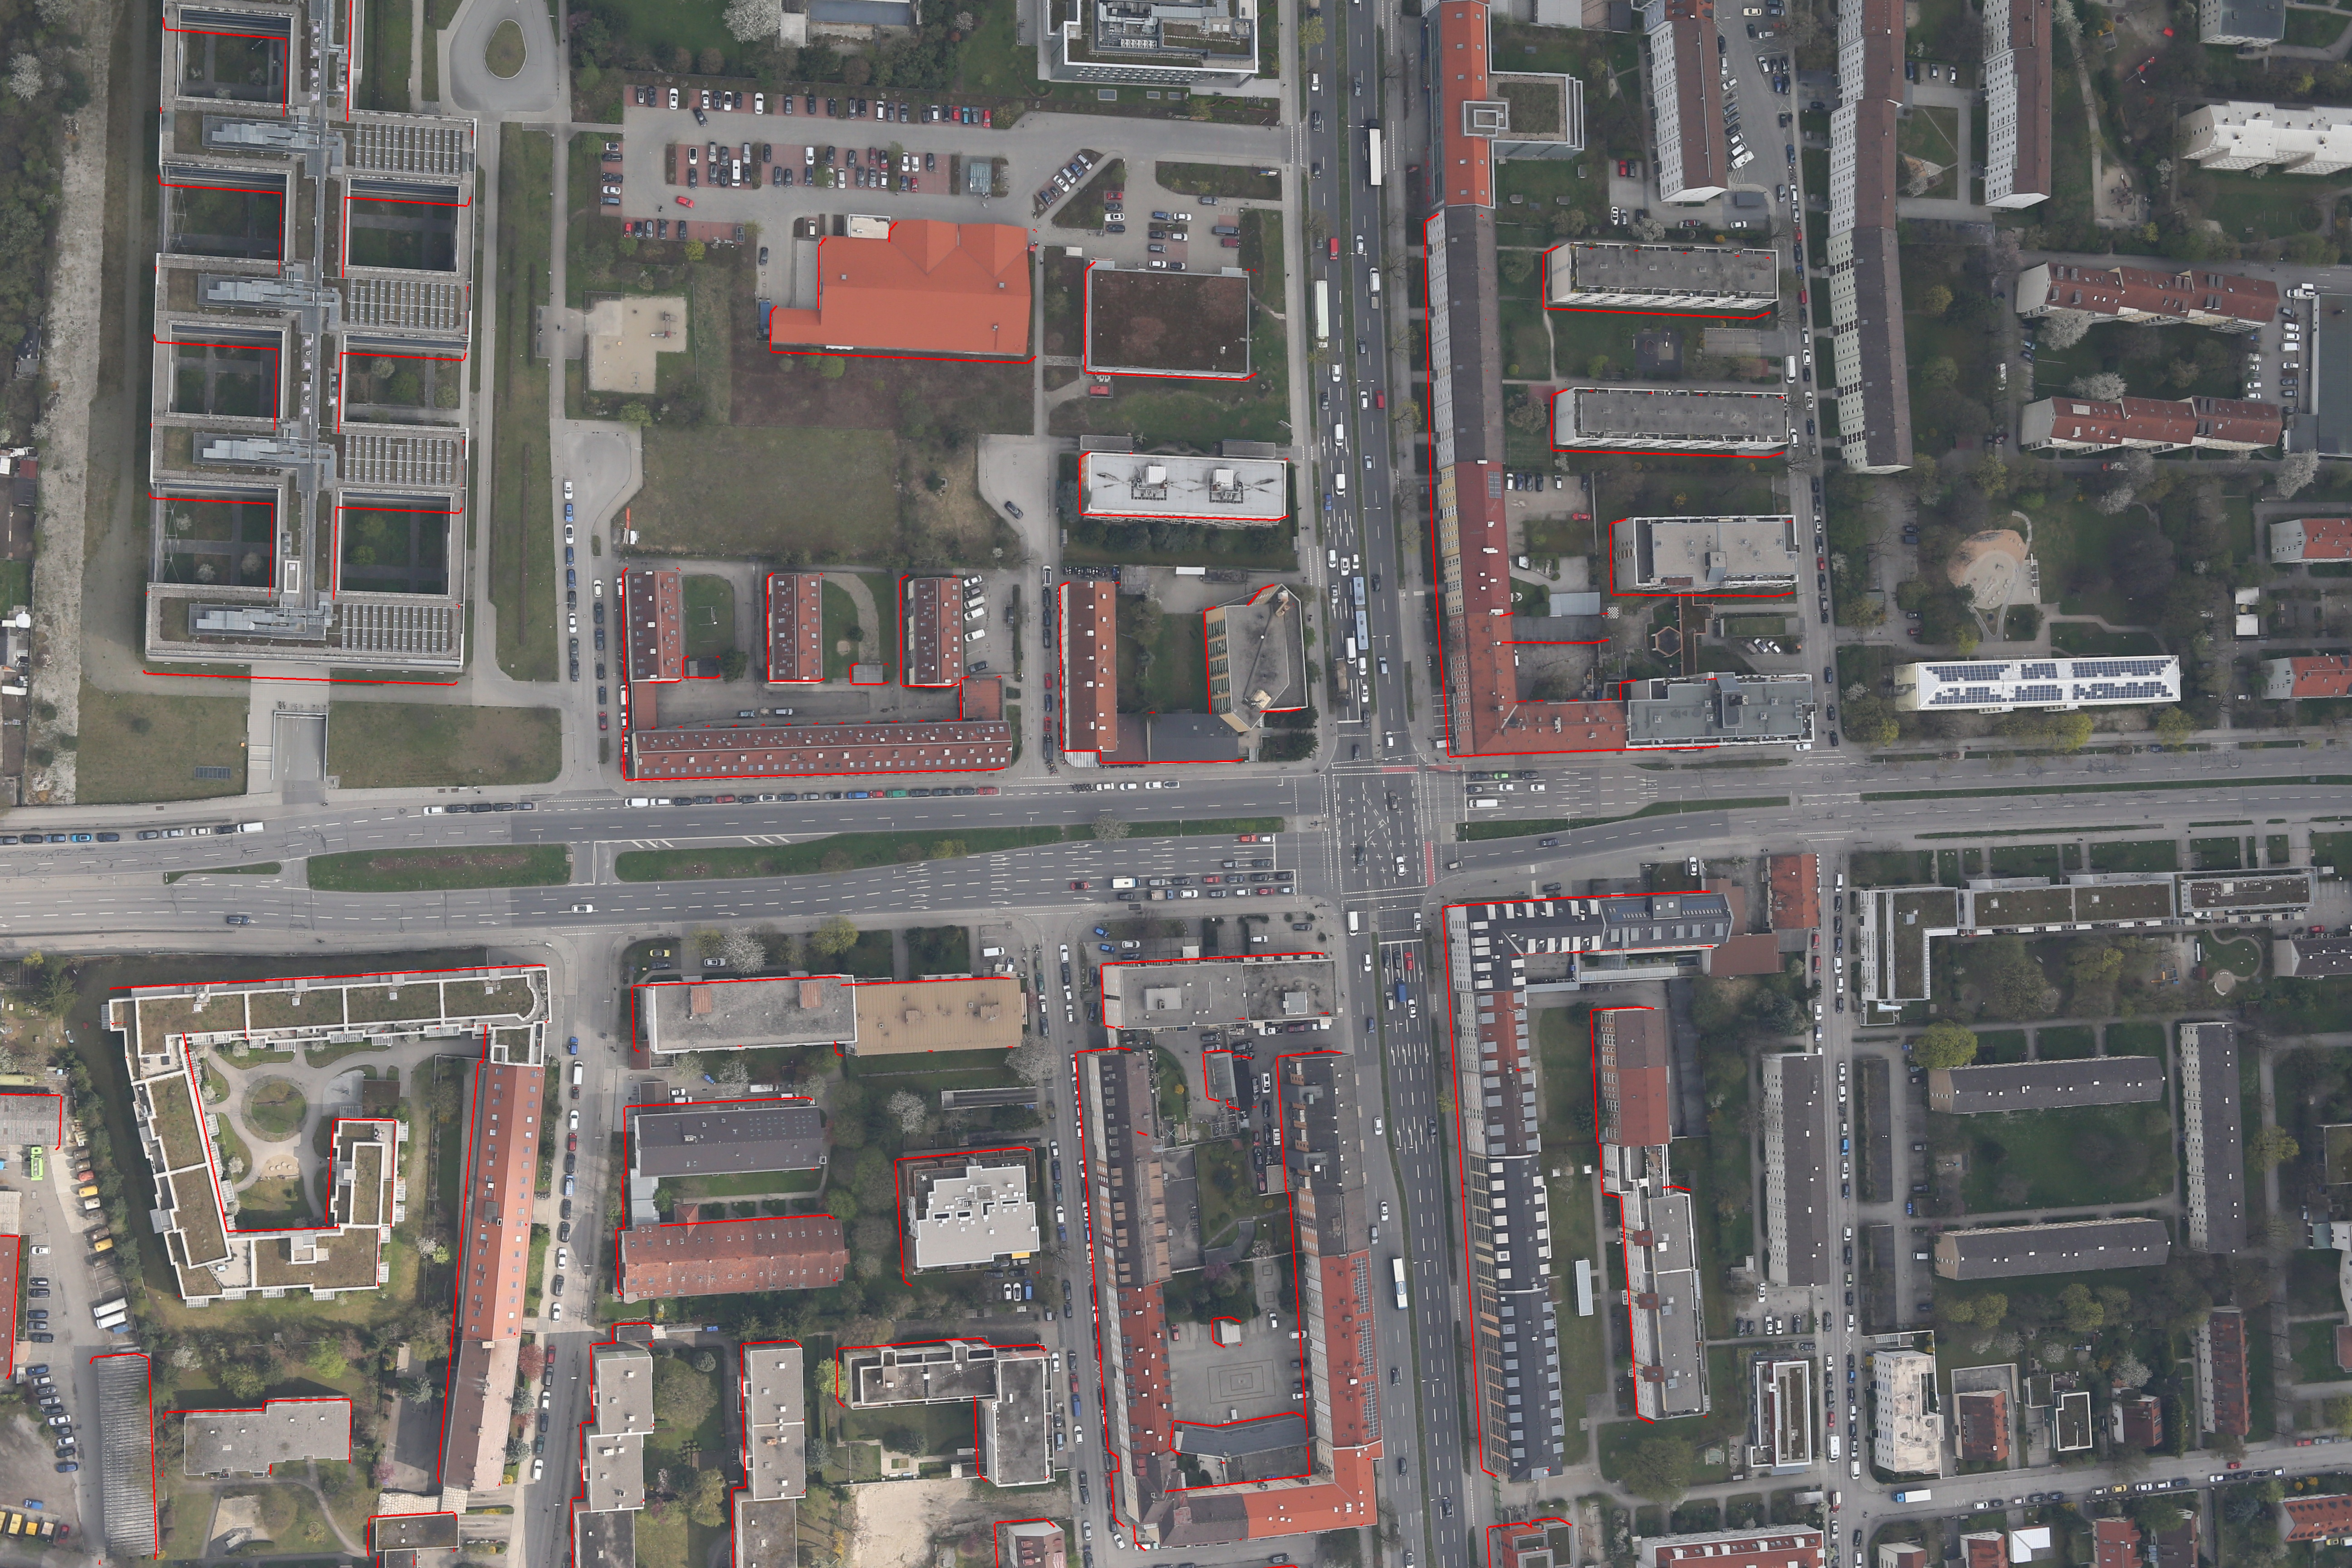
\includegraphics[width=\textwidth]{analysis/optimizable_3k.png}
           \caption[]{}
           {{\small }}
           \label{fig:3b}
       \end{subfigure}
       \begin{subfigure}[tbp]{0.9\columnwidth}
           \centering
           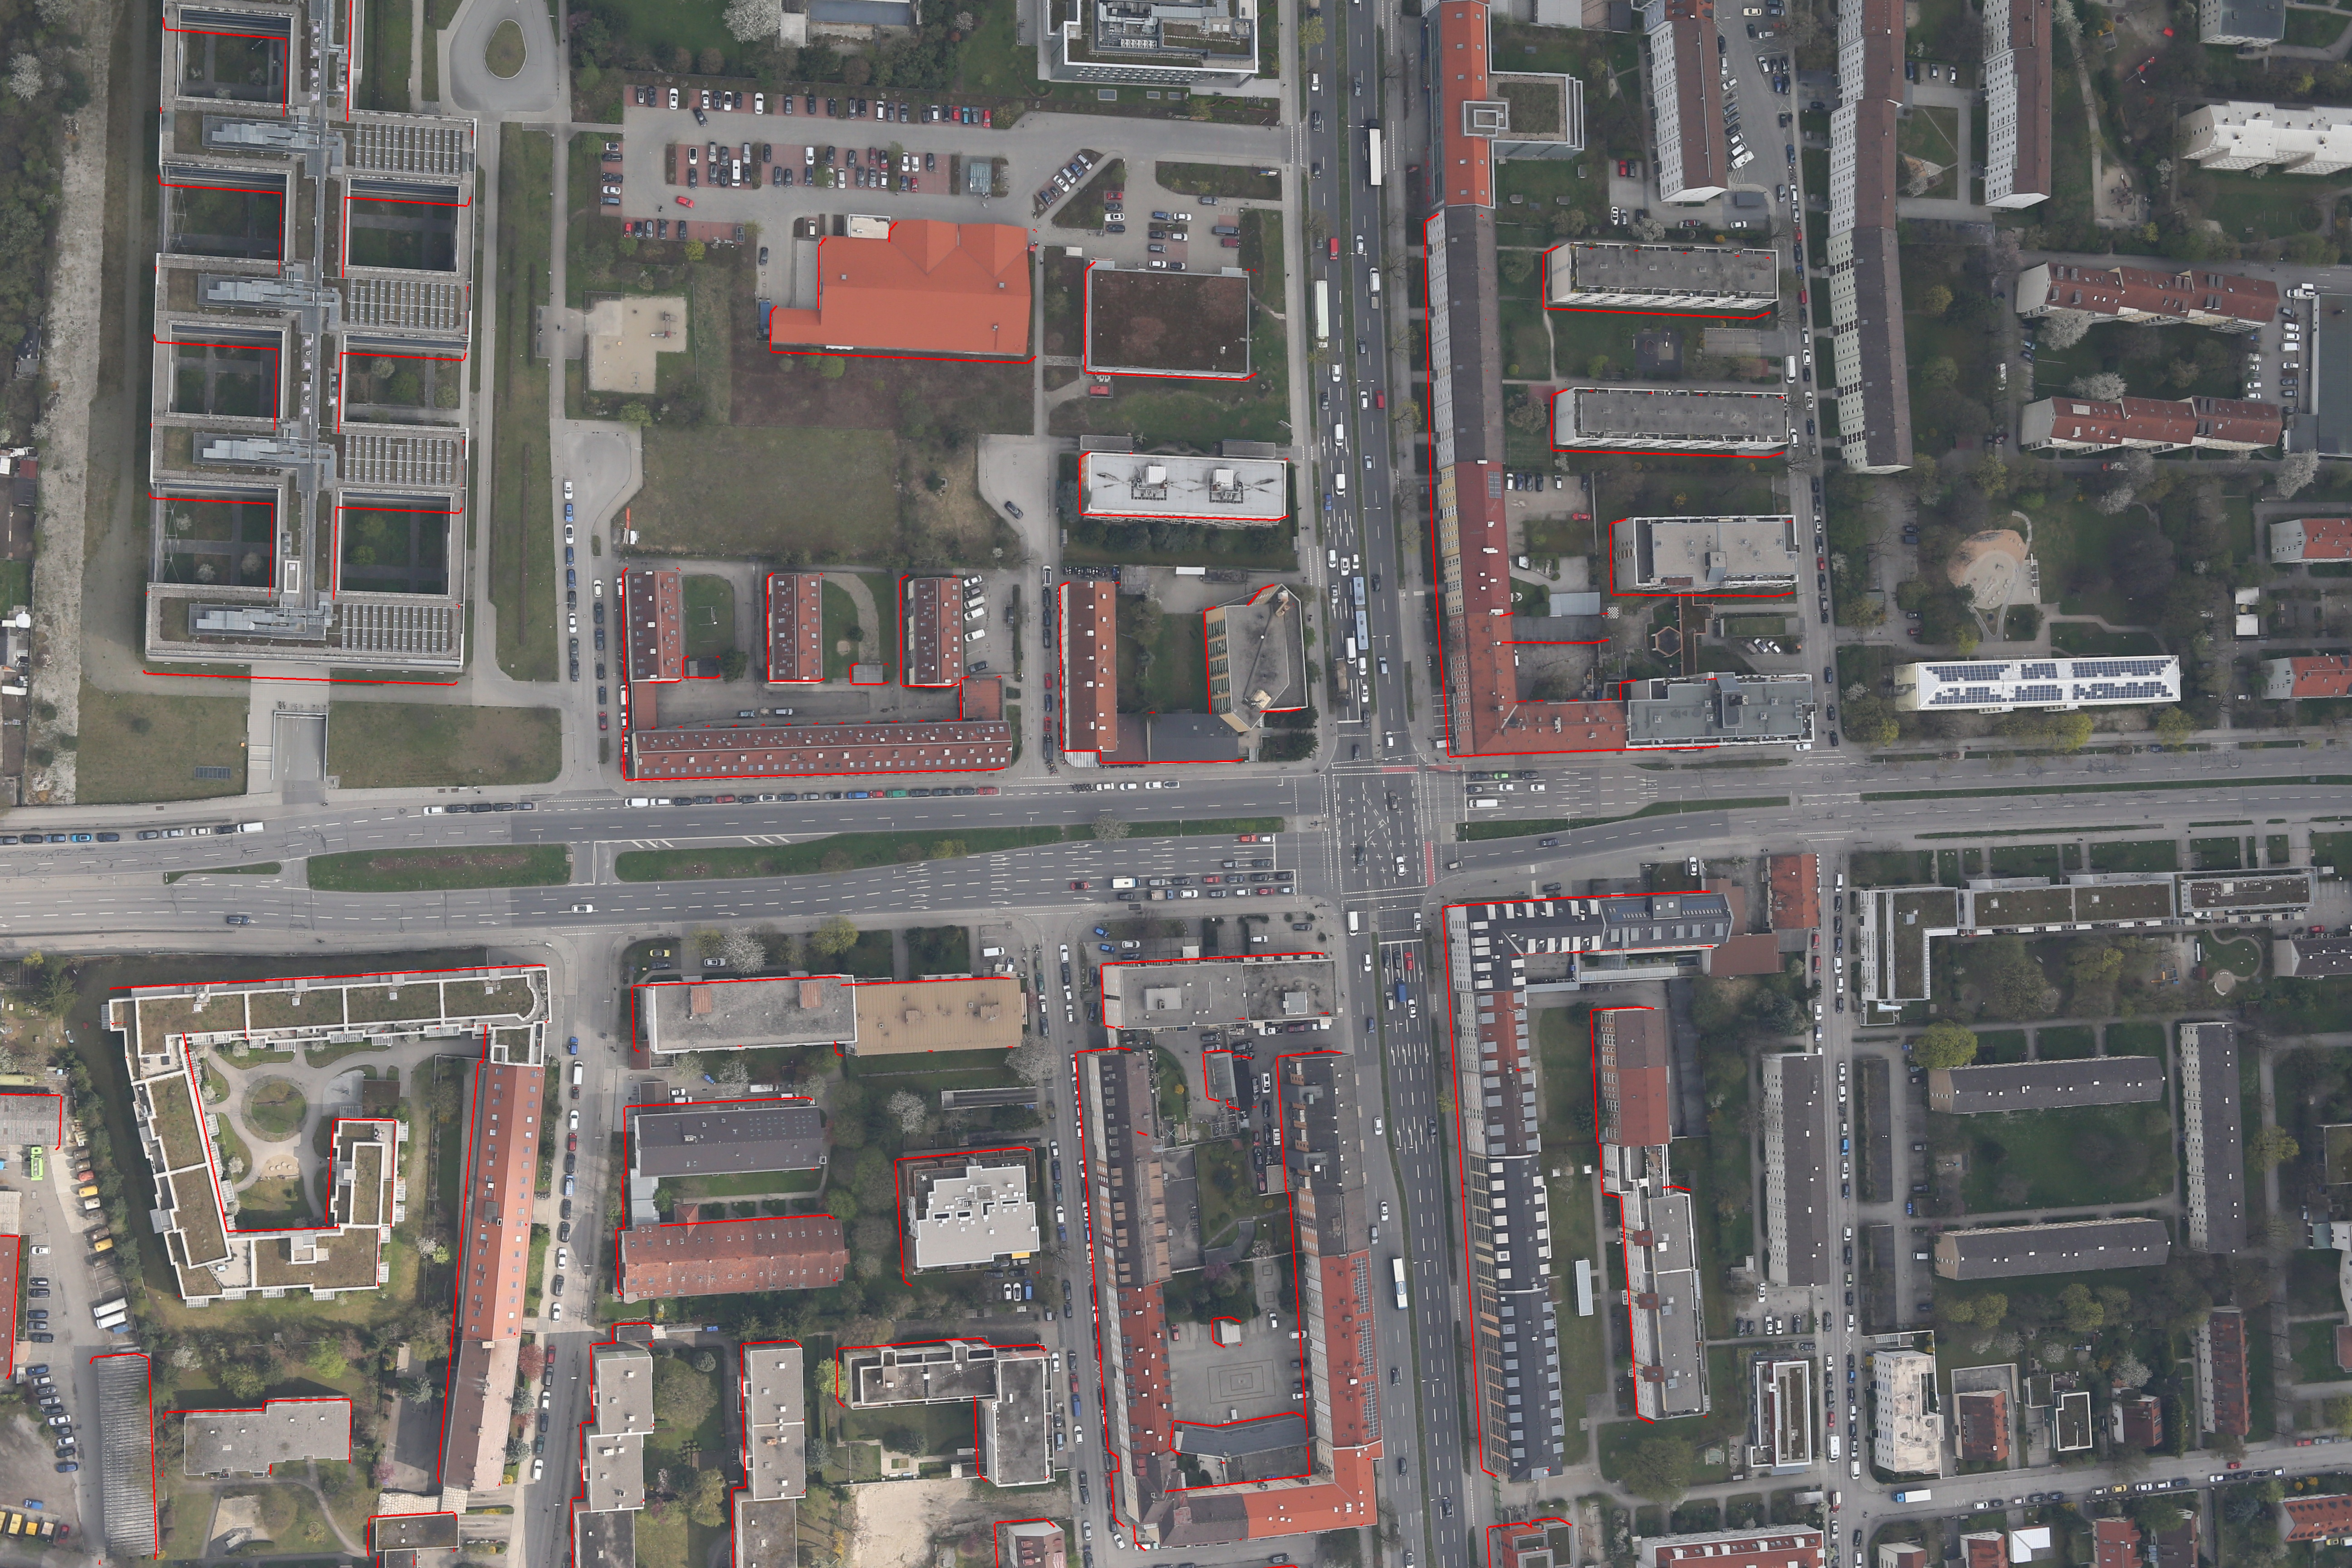
\includegraphics[width=\textwidth]{analysis/optimizable_3k.jpg}
           \caption[]{}
           {{\small }}
           \label{fig:3c}
       \end{subfigure}
       \vspace{-12pt}
\caption{Overview of optimizable building vertices in the presence of occlusions. Red lines are the projection of original OSM building footprints before optimization, highlighting the building edges that can be optimized.}
       \label{fig:optimizable}
\end{figure}


\section{Experiments}\label{sec:exp}
\hl{In order to validate the generalization ability of the proposed method, we test the methodology on four datasets with different building types. Furthermore, we compare the optimization results with the reference data. Qualitative and quantitative analyses are carried out to verify the accuracy of the optimized building footprint and height.} 
\subsection{Data Description}
\begin{itemize}
\item \textbf{Image data}
\end{itemize}

We collect images from four scenarios containing different types of buildings. \hl{The main characteristics of the datasets are listed in Table }% add reference of Table 1
\ref{tab:dataset}. In particular, Scenario A is targeted at optimization of footprints of individual buildings. To this end, 375 oblique images of an isolated cabin were captured by a UAV flight. The survey site lies on a bare agricultural land in Finning, Germany. Here, the building of interest is free from occlusions. The images were acquired by a Canon EOS-1DX camera mounted on a~rotary wing platform at altitudes ranging from 20 m to 50 m above ground and with pitch angle of $40\sim50^\circ$. The average ground sampling distance is 0.96 cm.

Scenario B presents a small kindergarten surrounded by trees and bushes in Oberpfaffenhofen, Germany. The dataset also serves for optimization of a footprint of an individual building, yet the scene is more complex with the presence of occlusions and shades. 142 images were acquired by a~Canon EOS-1DX camera, including 32 nadir-view images and 110 oblique-view images with a pitch angle of about $45^\circ$. The flight height ranges from 20 m to 45 m above ground, resulting in an average Ground Sampling Distance (GSD) of 1.09 cm. 

In addition, we also exploit the possibility to optimize footprints of multiple buildings. With~the increasing popularity of UAVs, more and more people are able to take photos or videos using their own drones and spontaneously share the data on the Internet with free access. In this context, Scenario C was established by extracting a series of frames from a YouTube video captured by a drone. The survey site is located in an urban residential area in Munich, Germany, containing many modern buildings, and most of them are partially occluded. The flight height is estimated to 40 m above ground with pitch angle around $40^\circ$. In total, 169 images with a GSD at image centers of 14.33 cm were extracted for the experiment. Each building can be visible or partly visible in 24--86 images, depending on its location in the survey area. It has to be noted that the low image resolution and the presence of occlusions cause difficulties for the subsequent optimization step.

Scenario D is an open dataset provided by \hl{the company senseFly} \cite{sullens}. The 37 oblique images were collected in a small village in Switzerland, featuring many traditional-style buildings surrounded or occluded by vegetation. Each building can be visible or partly visible in 31--37 images. The images were taken by a~Canon PowerShot camera from about 100 m above the ground with a pitch angle of $-50^\circ$, and the average image GSD is 5.46 cm. 

\begin{itemize}
\item \textbf{OSM data}
\end{itemize}

The OSM data used in experiments have been downloaded on 21 January 2018. The footprints contain only the planar coordinates of building footprints but no height information. According to the detailed quality assessment for OSM building footprints data \cite{fan2014quality}, the OSM footprints in our survey area (Munich) have a high completeness accuracy and a position accuracy of about 4 m in average. Therefore, they can be safely adopted to initialize a building model. 

\begin{itemize}
\item \textbf{Reference data}
\end{itemize}

For evaluation of the experimental results, we take the German ATKIS (Amtliches Topographisch-Kartographisches Informationssystem) data as reference. ATKIS has been developed as a common project of the Working Committees of the Survey Administrations of the States of the Federal Republic of Germany (AdV), containing information of objects of the `Real World' like roads, rivers or woodland \cite{atkis2000}. The position accuracy of building footprint in ATKIS is $\pm0.5$ m \cite{muller1998quality}. It needs to be pointed out that ATKIS data is not available to the public in Germany, therefore we can only request the ATKIS footprint data for small areas as ground truth. Specifically, the ATKIS data used in the experiments were published on 27 January 2016 and the building data is formatted as LoD1 CityGML model, i.e., the value of building height describes the difference in meters between the highest point of the roof and the ground. 

\begin{table}[H]
  \begin{center}
  \footnotesize 
  \begin{tabular}{@{}v{.09\linewidth}*{8}{c}@{}}
    \toprule
    \multicolumn{1}{@{}c}{\textbf{Dataset}} & \multicolumn{7}{c@{}}{\textbf{UAV Image}} \\
    \cmidrule{2-8} &    
    \multicolumn{1}{V{.08\linewidth}}{\centering\textbf{Date}}  &
    \multicolumn{1}{V{.12\linewidth}}{\centering\textbf{Resolution (pix)}} & 
    \multicolumn{1}{V{.08\linewidth}}{\centering\textbf{Height (m)}}  &
    \multicolumn{1}{V{.09\linewidth}}{\centering\textbf{Pitch Angle}}  &
    \multicolumn{1}{V{.08\linewidth}}{\centering\textbf{GSD (cm)}}&
    %Define if appropriate
    \multicolumn{1}{V{.15\linewidth}}{\centering\textbf{Number of Images per Building}}&
    \multicolumn{1}{V{.15\linewidth}}{\centering\textbf{Registration}} \\ 

    \cmidrule(){1-8}
    A &  10/2016 & $5184 \times 3456$ & 20 - 50 & 40--$50^{\circ}$ & 0.96 & 375 & MA \\ %375
    B &  10/2016 & $5184 \times 3456$ & 20 - 45 & $45^{\circ} , 90^{\circ}$ & 1.09 & 142 & AA  \\ %
    C &  01/2016 & $1296 \times 728$ & 40 & $50^{\circ}$ & 14.33 & 24--86 & MA  \\ %
    D &  06/2014 & $4000 \times 3000$ & 100 & $50^{\circ}$  & 5.46 & 31--37 & MA  \\ %37images
  \bottomrule
  \end{tabular}
  \end{center}
  \caption {Characteristics of the datasets used in the experiment. AA: automatically co-registered to aerial data; MA: manually co-registered to aerial data; -: pre-georeferenced.}
\label{tab:dataset}
\end{table}

\subsection{Geo-Registration of UAV Images}
Due to payload limitations, UAVs are usually equipped with low-quality GNSS/IMUs and can therefore achieve a direct geo-referencing accuracy of merely 3--5 m. To improve the position accuracy of OSM building footprints, however, UAV images are expected to have higher accuracy than OSM. To this end, we made various attempts at improving the geo-registration accuracy of UAV images. In particular, Scenarios A, C and D are manually geo-registered using measurements from geo-spatial products that have higher accuracy than the OSM data, whereas Scenario B is geo-registered to aerial images in a fully automated way.
% Though on-board GPS/IMU information is available in \texttt{Scenario A}, the accuracy is not sufficient for our application. In order to improve the absolute geo-referencing accuracy of UAV images,

For Scenario A, we manually established some \hl{GCPs}, whose planar coordinates ($x$,$y$) were measured on Bavaria DOP80 (\hl{digital orthophoto of 80 cm resolution, provided by Bavarian State Office for Survey and Geoinformation in Germany)} and the elevation values $z$ were extracted from DTK25 (\hl{Digital Topographic Model [DTM] of 25cm resolution, provided by Bavarian State Office for Survey and Geoinformation in Germany}). 
%Define if appropriate
These GCPs were then used to geo-register the UAV images dataset. Similarly, Scenario B was geo-registered using the GCPs measured from the orthophoto and DTM \cite{d2011semiglobal} reconstructed from the aerial images acquired by the DLR 3K camera system with cm-level accuracy \cite{kurz2014performance}. In Scenario D, GCPs were measured on \hl{SWISSIMAGE 25 (digital orthophoto of 25 cm resolution)} and swissNAMES3D (Topographical Landscape Model [TLM] of 0.2$\sim$1.5 m accuracy).

Scenario B contains both nadir-view and oblique-view UAV images. Here, the corresponding nadir-view aerial images with cm-level global accuracy are also available, thus we co-registered the low-accuracy UAV images to the high-accuracy aerial images following the approach proposed in \cite{zhuo2017automatic}. More specifically, we first solve the camera poses of the UAV images via Structure From Motion (SFM), and then match the nadir UAV images with nadir aerial images using the proposed matching scheme, resulting in thousands of reliable image correspondences. Since the aerial images are pre-georeferenced, 3D coordinates of those common image correspondences can be derived via image-to-ground projection of the aerial images, and these 3D points are then adopted to estimate the camera poses of the corresponding nadir-view UAV images. In the end, those UAV images with known camera poses are involved in a global optimization for camera poses of all UAV images. In this way, all UAV images get geo-registered.

We used the software \hl{Pix4Dmapper Pro (version 4.0.25)} for the process and orientation of the UAV data. The mean reprojection errors of the four datasets are in the range of 0.15--0.2 pixels.

% \begin{figure}[H]
%     \centering
%        \begin{subfigure}[tbp]{0.24\columnwidth}
%            \centering
%            \includegraphics[width=\textwidth]{reconstruction/match.jpg}
           
%            {{\small }}
%            \label{fig:match}
%        \end{subfigure}
%        \caption{Example of matching UAV image with reference aerial image}       
%        \label{fig:geo-register}
% \end{figure}

\subsection{Semantic Image Segmentation Using CRFasRNN}
For a robust and generalized training of the neural network, we collect training images evenly distributed from the four datasets, to ensure that different types of buildings are all included in the training dataset. The training images were manually labeled with seven categories: building, roof, ground, road, vegetation, vehicle and clutter. Among them, categories like building, roof and ground are of most interest for our application. In order to compensate for the shortage of training data, we~implemented data augmentation by cropping, rotating and scaling the training data. Around 10,000 annotated images with a size of 300 $\times$ 300 pixels were generated for training.


The deep learning procedure was implemented under the framework Caffe \cite{jia2014caffe}. Instead of training the network from scratch, we fine-tuned the FCN-8s PASCAL model from the Berkeley Vision and Learning Center (BVLC) on our own dataset. As the boundary between different classes is of interest for our application, we plugged in the CRF-RNN layer in order to achieve sharp edges at class borders. The training process started to converge at iteration 6000 and was stopped at iteration 74,000 before over-fitting. Figure \ref{fig:seg} depicts the segmentation results of the trained network on the test data. Figure \ref{fig:seg}a,b are test images from Scenario A, while Figure \ref{fig:seg}e,f are the segmentation results. It can be seen that the roofs, fa\c{c}ades, building and the surrounding clutter are basically correctly segmented; Figure \ref{fig:seg}c,d,g,h are respectively the original and segmented images from Scenario D, the segmentation in building areas is noisy due to shading and poor illumination. Figure \ref{fig:seg}i--p in the last two rows display segmentation results from Scenarios C and D with multiple buildings. 

To conclude, despite a few incorrect segmentations in areas with complex textures or structures, the~overall segmentation achieved a remarkable performance and yielded reliable image labels. 

\begin{figure}[H]
    \centering
       \begin{subfigure}[tbp]{0.24\columnwidth}
           \centering
           \includegraphics[width=\textwidth]{segment/fin_ori1.png}
           \caption[]{}
           {{\small }}
           \label{fig:4a}
       \end{subfigure}
       \begin{subfigure}[tbp]{0.24\columnwidth}
           \centering
           \includegraphics[width=\textwidth]{segment/fin_ori2.png}
           \caption[]{}%
           {{\small }}
           \label{fig:4b}
       \end{subfigure}
       \hfill
       \begin{subfigure}[tbp]{0.24\columnwidth}
           \centering
           \includegraphics[width=\textwidth]{segment/kiga_ori1.png}
           \caption[]{}
           {{\small }}
           \label{fig:4c}
       \end{subfigure}       
       \begin{subfigure}[tbp]{0.24\columnwidth}
           \centering
           \includegraphics[width=\textwidth]{segment/kiga_ori2.png}
           \caption[]{}%
           {{\small }}
           \label{fig:4d}
       \end{subfigure}
       \hfill       
       \begin{subfigure}[tbp]{0.24\columnwidth}  
           \centering 
           \includegraphics[width=\textwidth]{segment/fin_seg1.png}
           \caption[]{}
           {{\small }}    
           \label{fig:4e}
       \end{subfigure}       
       \begin{subfigure}[tbp]{0.24\columnwidth}  
           \centering 
           \includegraphics[width=\textwidth]{segment/fin_seg2.png}
           \caption[]{}%
           {{\small }}    
           \label{fig:4f}
       \end{subfigure}
       \hfill
       \begin{subfigure}[tbp]{0.24\columnwidth}  
           \centering 
           \includegraphics[width=\textwidth]{segment/kiga_seg1.png}
           \caption[]{}
           {{\small }}    
           \label{fig:4g}
       \end{subfigure}       
       \begin{subfigure}[tbp]{0.24\columnwidth}  
           \centering 
           \includegraphics[width=\textwidth]{segment/kiga_seg2.png}
           \caption[]{}%
           {{\small }}    
           \label{fig:4h}
       \end{subfigure} 
       \begin{subfigure}[tbp]{0.275\columnwidth}
           \centering
           \includegraphics[width=\textwidth]{segment/mil_ori1.png}
           \caption[]{}
           {{\small }}
           \label{fig:4i}
       \end{subfigure}
       \begin{subfigure}[tbp]{0.275\columnwidth}
           \centering
           \includegraphics[width=\textwidth]{segment/mil_ori2.png}
           \caption[]{}%
           {{\small }}
           \label{fig:4j}
       \end{subfigure}
       \hfill
       \begin{subfigure}[tbp]{0.21\columnwidth}
           \centering
           \includegraphics[width=\textwidth]{segment/sullens_ori1.png}
           \caption[]{}
           {{\small }}
           \label{fig:4k}
       \end{subfigure}
       \begin{subfigure}[tbp]{0.21\columnwidth}
           \centering
           \includegraphics[width=\textwidth]{segment/sullens_ori2.png}
           \caption[]{}%
           {{\small }}
           \label{fig:4l}
       \end{subfigure}
       \begin{subfigure}[tbp]{0.275\columnwidth}  
           \centering 
           \includegraphics[width=\textwidth]{segment/mil_seg1.png}
           \caption[]{}
           {{\small }}    
           \label{fig:4m}
       \end{subfigure}       
       \begin{subfigure}[tbp]{0.275\columnwidth}  
           \centering 
           \includegraphics[width=\textwidth]{segment/mil_seg2.png}
           \caption[]{}%
           {{\small }}    
           \label{fig:4n}
       \end{subfigure}
       \hfill
       \begin{subfigure}[tbp]{0.21\columnwidth}  
           \centering 
           \includegraphics[width=\textwidth]{segment/sullens_seg1.png}
           \caption[]{}
           {{\small }}    
           \label{fig:4o}
       \end{subfigure}       
       \begin{subfigure}[tbp]{0.21\columnwidth}  
           \centering 
           \includegraphics[width=\textwidth]{segment/sullens_seg2.png}
           \caption[]{}%
           {{\small }}    
           \label{fig:4p}
      \end{subfigure}
      \protect\includegraphics[scale=1]{fig1.pdf}\quad
      \protect\includegraphics[scale=1]{fig2.pdf}\quad
      \protect\includegraphics[scale=1]{fig3.pdf}\quad
      \protect\includegraphics[scale=1]{fig4.pdf}\quad
      \protect\includegraphics[scale=1]{fig5.pdf}\quad
      \protect\includegraphics[scale=1]{fig6.pdf}\quad
      \protect\includegraphics[scale=1]{fig7.pdf}
%       \fcolorbox{red}{red}{\rule{0pt}{5pt}\rule{13pt}{0pt}} roof \quad
%       \fcolorbox{blue}{blue}{\rule{0pt}{5pt}\rule{13pt}{0pt}} building \quad  
%       \fcolorbox{gray}{gray}{\rule{0pt}{5pt}\rule{13pt}{0pt}} ground  \quad 
%       \fcolorbox{gray}{myroad}{\rule{0pt}{5pt}\rule{13pt}{0pt}} road  \quad
%\fcolorbox{green}{green}{\rule{0pt}{5pt}\rule{13pt}{0pt}}  vegetation  \quad
%       \fcolorbox{yellow}{yellow}{\rule{0pt}{5pt}\rule{13pt}{0pt}}  vehicle  \quad
%       \fcolorbox{black}{black}{\rule{0pt}{5pt}\rule{13pt}{0pt}}  clutter       
       \caption{Segmentation results of four scenarios. (\textbf{a}) and (\textbf{b}) are test images of Scenario A while (\textbf{e}) and (\textbf{f}) are corresponding segmentation results; (\textbf{c}) and (\textbf{d}) are test images of Scenario B while (\textbf{g}) and (\textbf{h}) are corresponding segmentation results; (\textbf{i}) and (\textbf{j}) are test images of Scenario C while (\textbf{m}) and (\textbf{n}) are corresponding segmentation results; (\textbf{k}) and (\textbf{l}) are test images of Scenario D while (\textbf{o}) and (\textbf{p}) are corresponding segmentation results.}       
       \label{fig:seg}
\end{figure}

\subsection{OSM Building Footprint Optimization}
As we regard the building boundaries extracted from the segmented images as a constraint for optimization, it is crucial that the image segmentation, at least for the building and its surroundings, should yield accurate and reliable results. In practice, however, there are inevitably some poorly segmented images in a dataset, thus we need to select those images that satisfy those requirements: 
\begin{enumerate}[leftmargin=*,labelsep=5.5mm]
\item The segmented building areas have accurate boundaries; 
\item Buildings are not occluded by vegetation or obstacles;
\item The selected images are expected to be taken from different viewpoints so that all vertices of the building footprint can be optimized.
\end{enumerate}
  


Figure \ref{fig:refine} demonstrates the results of footprint optimization process. Figure \ref{fig:refine}a--c are projections of original OSM footprints with the height extracted from DSM, while Figure \ref{fig:refine}d--f are projections of the optimized building sketch of Scenario A. Figure \ref{fig:refine}g,h are projections of original OSM footprints with the height extracted from DSM, while Figure \ref{fig:refine}j,k are projections of the optimized building sketch of Scenario B. Figure \ref{fig:refine}i,l illustrate a combined footprint of two adjacent buildings with different heights before and after optimization, therefore only the footprint get optimized. The original projections of the footprints extracted from OSM with the height from DSM are highlighted by the red lines, which have large position shift with respect to the building. The projections of the footprints after optimization using the proposed method are marked by blue lines, which fit precisely the building borders. It is evident that the image projection accuracy of the optimized footprints have improved conspicuously compared to the original OSM footprints. 


\begin{figure}[H]
    \centering
       \begin{subfigure}[tbp]{0.31\columnwidth}
           \centering
           \includegraphics[width=\textwidth]{optimize/IMG_0735_osm_ori.png}
           \caption[]{}%
           {{\small }}
           \label{fig:5a}
       \end{subfigure} 
       \begin{subfigure}[tbp]{0.31\columnwidth}  
           \centering 
           \includegraphics[width=\textwidth]{optimize/IMG_0765_osm_ori.png}
           \caption[]{}%
           {{\small }}    
           \label{fig:5b}
       \end{subfigure}
       \begin{subfigure}[tbp]{0.31\columnwidth}  
           \centering 
           \includegraphics[width=\textwidth]{optimize/IMG_0951_osm_ori.png}
           \caption[]{}%
           {{\small }}   
           \label{fig:5c}
       \end{subfigure}
       
       \begin{subfigure}[tbp]{0.31\columnwidth}
           \centering
           \includegraphics[width=\textwidth]{optimize/IMG_0735_xyzh.png}
           \caption[]{}%
           {{\small }}
           \label{fig:5d}
       \end{subfigure}
       \begin{subfigure}[tbp]{0.31\columnwidth}  
           \centering 
           \includegraphics[width=\textwidth]{optimize/IMG_0765_xyzh.png}
           \caption[]{}%
           {{\small }}    
           \label{fig:5e}
       \end{subfigure}
       \begin{subfigure}[tbp]{0.31\columnwidth}  
           \centering 
           \includegraphics[width=\textwidth]{optimize/IMG_0951_xyzh.png}
           \caption[]{}%
           {{\small }}   
           \label{fig:5f}
       \end{subfigure} 
       \begin{subfigure}[tbp]{0.31\columnwidth}
           \centering
           \includegraphics[width=\textwidth]{optimize/IMG_1367_xy.png}
           \caption[]{}%
           {{\small }}
           \label{fig:5g}
       \end{subfigure}
       \begin{subfigure}[tbp]{0.31\columnwidth}  
           \centering 
           \includegraphics[width=\textwidth]{optimize/IMG_1604_xy.png}
           \caption[]{}%
           {{\small }}    
           \label{fig:5h}
       \end{subfigure}
       \begin{subfigure}[tbp]{0.31\columnwidth}  
           \centering 
           \includegraphics[width=\textwidth]{optimize/IMG_1400_osm_ori.png}
           \caption[]{}%
           {{\small }}   
           \label{fig:5i}
       \end{subfigure}
       \begin{subfigure}[tbp]{0.31\columnwidth}
           \centering
           \includegraphics[width=\textwidth]{optimize/IMG_1367_xyzh.png}
           \caption[]{}%
           {{\small }}
           \label{fig:5j}
       \end{subfigure}
       \begin{subfigure}[tbp]{0.31\columnwidth}  
           \centering 
           \includegraphics[width=\textwidth]{optimize/IMG_1604_xyzh.png}
           \caption[]{}%
           {{\small }}    
           \label{fig:5k}
       \end{subfigure}
       \begin{subfigure}[tbp]{0.31\columnwidth}  
           \centering 
           \includegraphics[width=\textwidth]{optimize/IMG_1400_xyzh.png}
           \caption[]{}%
           {{\small }}   
           \label{fig:5l}
       \end{subfigure}       
      
       \caption{Image projections of building sketch before and after optimization. Red lines are projections of original OSM footprints with height measured from DSM, blue lines show projections of optimized building footprints and heights, and the green line shows a combined footprint for two buildings with different height.}
       \label{fig:refine}
\end{figure}


For the visualization of the absolute position accuracy of the optimized footprints, we overlap the footprints before and after optimization together with ATKIS data. As shown in Figure \ref{fig:overlay}, the gray areas are reference footprints from ATKIS data, red lines indicate original footprints extracted from OSM, and blue lines show the footprints after optimization using the proposed method. All footprints are overlapped together in the same coordinate reference system. To be specific, Figure \ref{fig:overlay}a shows the footprints of the two cabins from Scenario A. All corners of the larger building on the right get optimized with a significant improvement in position accuracy. It should be pointed out that the smaller building on the left is not our main target and therefore only appears in a few images, still all its three visible corners got optimized with satisfying accuracy. Figure \ref{fig:overlay}b shows the footprints of a house from Scenario B, which is composed of two small adjacent houses. The building footprint in OSM, however, is simplified to a rectangular shape with a large position shift. As a correct hypothesis of the building shape is the prerequisite for reasonable optimization, we extracted eight corners of the roof based on the corresponding orthophoto and DSM. The new building footprint, colored in green in Figure \ref{fig:overlay}b, was used as the initial value for optimization. The optimized footprint, highlighted in blue, matches the reference data well. The experimental results demonstrate that, given the correct hypothesis of the building shape, our method is able to efficiently optimize the footprint of individual buildings even if the initial values are far from accurate.


\begin{figure}[H]
    \centering
\begin{subfigure}[tbp]{0.47\columnwidth}
           \centering
           \includegraphics[height=4cm]{optimize/finning_overlay.png}
           \caption[]{}
           {{\small }}
           \label{fig:6a}
       \end{subfigure}
       \begin{subfigure}[tbp]{0.47\columnwidth}
           \centering
           \includegraphics[height=4cm]{optimize/kiga_overlay.png}
           \caption[]{}%
           {{\small }}
           \label{fig:6b}
       \end{subfigure}
       \caption{Optimization for multiple buildings. (\textbf{a}) and (\textbf{b}) show the result of Scenario A Scenario B respectively; gray areas represent the reference footprints from ATKIS 
%Define if appropriate       
data, red lines indicate original footprints extracted from OSM, blue lines show the footprints after optimization using the proposed method, and green represents the initial lines for optimization.}
       \label{fig:overlay}
\end{figure}

In contrast, Scenario C and Scenario D feature multiple buildings that are partly occluded. \mbox{As a consequence}, only the visible building corners may get optimized. In addition, the performance of optimization is also affected by the quality of image segmentation. 

\hl{Figure} \ref{fig:optimized}a,b illustrate the optimization results of Scenario C. Blue lines indicate an overall projection of all optimized buildings, while the optimization for the rest of the buildings failed as a result of severe occlusions or poor segmentation. It can be seen that more than half of the visible building corners were successfully optimized despite the low image resolution, and the estimated building height aligns well with the border between the roof and the building.

Within Scenario D, most buildings are surrounded by thick vegetation, and we extract only the boundary between the ground and the building. For that reason, there are few effective contours available for optimization. Figures \ref{fig:optimized}c--f show some of the optimized building footprints, where the red lines correspond to the original OSM building footprints and blue lines refer to the optimized building footprints. It should be noted that the OSM footprints data for rural areas exhibit much larger errors than in the urban area. Nevertheless, our method still achieves accurate optimization results for visible building edges.



\begin{figure}[H]
    \centering
       \begin{subfigure}[tbp]{0.48\columnwidth}
           \centering
           \includegraphics[width=\textwidth]{optimize/mil_alloptim_1.png}
           \caption[]{}
           {{\small }}
           \label{fig:7a}
       \end{subfigure}
       \hfill
       \begin{subfigure}[tbp]{0.48\columnwidth}
           \centering
           \includegraphics[width=\textwidth]{optimize/mil_alloptim_2.png}
           \caption[]{}
           {{\small }}
           \label{fig:7b}
       \end{subfigure}
       \hfill
       \begin{subfigure}[tbp]{0.24\columnwidth}
           \centering
           \includegraphics[height=2.8cm]{optimize/su_both_1.png}
           \caption[]{}
           {{\small }}
           \label{fig:7c}
       \end{subfigure}
       \hfill
       \begin{subfigure}[tbp]{0.24\columnwidth}
           \centering
           \includegraphics[height=2.8cm]{optimize/su_both_2.png}
           \caption[]{}
           {{\small }}
           \label{fig:7d}
       \end{subfigure} 
       \hfill
       \begin{subfigure}[tbp]{0.24\columnwidth}
           \centering
           \includegraphics[height=2.8cm]{optimize/su_both_3.png}
           \caption[]{}
           {{\small }}
           \label{fig:7e}
       \end{subfigure}
       \hfill
       \begin{subfigure}[tbp]{0.24\columnwidth}
           \centering
           \includegraphics[height=2.8cm]{optimize/su_both_4.png}
           \caption[]{}
           {{\small }}
           \label{fig:7f}
       \end{subfigure}         
       \caption{Optimization for multiple buildings. Red lines are the projections of the original OSM building footprints while blue lines correspond to the optimized building footprints; (\textbf{a}) and (\textbf{b}) give~an overall view of all the optimized buildings in Scenario C; (\textbf{c}) to (\textbf{f}) enumerate some of the optimized buildings of Scenario D.}
       
       \label{fig:optimized}
\end{figure}

\subsection{Accuracy Evaluation of Building Position and Height}
Apart from the visual comparison of the results, we performed a quantitative analysis of the results. Following the evaluation approach in \cite{fan2014quality}, we investigate the position accuracy of building footprints by calculating the average distance between the corresponding vertices pair from the optimized footprints and the reference data. In this sense, only the vertices appearing in both datasets can be compared.

In order to evaluate the optimization accuracy quantitatively, we compare the footprints before and after optimization with reference to ATKIS data. The results of Scenario A, B, and C are listed in Table \ref{tab:error_xy}. The second column lists the optimized buildings in each scenario, and for each building footprint, we manually measure the coordinates of each vertex and calculate the distance to the corresponding vertex in ATKIS data. The column Initial lists the errors in the \emph{x}- and \emph{y}-directions as well as the Euclidean distance of each vertex from the original footprint, whereas the column Optimized reports the errors of the optimized building footprint. Scenario C contains a number of optimizable buildings, from which six buildings with their optimized vertices are randomly selected as representatives. The~value average shows the average distance of all building vertices of each Scenario. 

Given that the building footprints in ATKIS have an average accuracy of $\pm{0.5}$ m, we can draw the conclusion that the accuracy of the building footprints has substantially increased after optimization using our method.

\begin{table}[H]
  \centering
  \caption{Position errors of building footprints before and after optimization. The column Initial lists the errors in the \emph{x}- and \emph{y}-directions as well as the Euclidean distance of each vertex of the original footprints; the column Optimized reports the errors of the optimized building footprints. }
    \begin{tabular}{cccccccc}
    \toprule
    \multirow{2}[2]{*}{\textbf{Scenario}} & \multirow{2}[2]{*}{\textbf{Building}} & \multicolumn{3}{c}{\textbf{Initial}} & \multicolumn{3}{c}{\textbf{Optimized}} \\
\cline{3-8}          &       & \multicolumn{1}{c}{\boldmath{$\Delta X$ \textbf{(m)}}} & \multicolumn{1}{c}{\boldmath{$\Delta Y$ \textbf{(m)}}} & \multicolumn{1}{c}{\textbf{Distance (m)}} & \multicolumn{1}{c}{\boldmath{$\Delta X$ \textbf{(m)}}} & \multicolumn{1}{c}{\boldmath{$\Delta Y$ \textbf{(m)}}} & \multicolumn{1}{c}{\textbf{Distance (m)}} \\
    \hline
    \multirow{8}[5]{*}{\vspace{8pt}A} & \multirow{4}[2]{*}{1} & \multicolumn{1}{c}{0.207} & \multicolumn{1}{c}{$-$1.213} & \multicolumn{1}{c}{1.230} & \multicolumn{1}{c}{0.623} & \multicolumn{1}{c}{$-$0.328} & \multicolumn{1}{c}{0.704} \\
          &       & \multicolumn{1}{c}{$-$0.374} & \multicolumn{1}{c}{0.942} & \multicolumn{1}{c}{1.014} & \multicolumn{1}{c}{0.145} & \multicolumn{1}{c}{0.427} & \multicolumn{1}{c}{0.451} \\
          &       & \multicolumn{1}{c}{1.601} & \multicolumn{1}{c}{1.545} & \multicolumn{1}{c}{2.225} & \multicolumn{1}{c}{0.020} & \multicolumn{1}{c}{0.137} & \multicolumn{1}{c}{0.139} \\
          &       & \multicolumn{1}{c}{2.247} & \multicolumn{1}{c}{$-$0.521} & \multicolumn{1}{c}{2.307} & \multicolumn{1}{c}{0.276} & \multicolumn{1}{c}{0.165} & \multicolumn{1}{c}{0.322} \\
\cline{2-8}          & \multirow{3}[2]{*}{2} & \multicolumn{1}{c}{1.733} & \multicolumn{1}{c}{1.157} & \multicolumn{1}{c}{2.084} & \multicolumn{1}{c}{0.233} & \multicolumn{1}{c}{0.657} & \multicolumn{1}{c}{0.697} \\
          &       & \multicolumn{1}{c}{2.114} & \multicolumn{1}{c}{$-$0.511} & \multicolumn{1}{c}{2.175} & \multicolumn{1}{c}{$-$0.164} & \multicolumn{1}{c}{$-$0.097} & \multicolumn{1}{c}{0.190} \\
          &       & \multicolumn{1}{c}{0.080} & \multicolumn{1}{c}{$-$0.899} & \multicolumn{1}{c}{0.902} & \multicolumn{1}{c}{0.655} & \multicolumn{1}{c}{$-$0.481} & \multicolumn{1}{c}{0.813} \\
\cline{2-8}          & average &       &       & \multicolumn{1}{c}{1.705} &       &       & \multicolumn{1}{c}{0.474} \\
    \hline
    \multirow{9}[4]{*}{B} & \multirow{8}[2]{*}{1} & \multicolumn{1}{c}{0.275} & \multicolumn{1}{c}{0.043} & \multicolumn{1}{c}{0.278} & \multicolumn{1}{c}{0.395} & \multicolumn{1}{c}{$-$0.037} & \multicolumn{1}{c}{0.397} \\
          &       & \multicolumn{1}{c}{0.758} & \multicolumn{1}{c}{1.337} & \multicolumn{1}{c}{1.537} & \multicolumn{1}{c}{0.118} & \multicolumn{1}{c}{$-$0.383} & \multicolumn{1}{c}{0.401} \\
          &       & \multicolumn{1}{c}{2.635} & \multicolumn{1}{c}{0.436} & \multicolumn{1}{c}{2.671} & \multicolumn{1}{c}{0.345} & \multicolumn{1}{c}{$-$0.074} & \multicolumn{1}{c}{0.353} \\
          &       & \multicolumn{1}{c}{2.756} & \multicolumn{1}{c}{$-$0.400} & \multicolumn{1}{c}{2.785} & \multicolumn{1}{c}{0.326} & \multicolumn{1}{c}{$-$0.100} & \multicolumn{1}{c}{0.341} \\
          &       & \multicolumn{1}{c}{2.848} & \multicolumn{1}{c}{$-$1.306} & \multicolumn{1}{c}{3.133} & \multicolumn{1}{c}{0.233} & \multicolumn{1}{c}{$-$0.008} & \multicolumn{1}{c}{0.233} \\
          &       & \multicolumn{1}{c}{$-$2.807} & \multicolumn{1}{c}{0.522} & \multicolumn{1}{c}{2.856} & \multicolumn{1}{c}{0.142} & \multicolumn{1}{c}{$-$0.102} & \multicolumn{1}{c}{0.175} \\
          &       & \multicolumn{1}{c}{$-$2.632} & \multicolumn{1}{c}{1.763} & \multicolumn{1}{c}{3.168} & \multicolumn{1}{c}{0.218} & \multicolumn{1}{c}{$-$0.227} & \multicolumn{1}{c}{0.314} \\
          &       & \multicolumn{1}{c}{0.342} & \multicolumn{1}{c}{0.461} & \multicolumn{1}{c}{0.574} & \multicolumn{1}{c}{0.192} & \multicolumn{1}{c}{$-$0.209} & \multicolumn{1}{c}{0.284} \\
\cline{2-8}          & average &       &       & \multicolumn{1}{c}{2.125} &       &       & \multicolumn{1}{c}{0.312} \\
    \hline
    \multirow{14}[14]{*}{\vspace{24pt}C} & \multirow{3}[1]{*}{1} & 0.039 & $-$2.073 & 2.073 & $-$0.029 & $-$0.682 & 0.683 \\
          &       & $-$0.078 & $-$1.927 & 1.928 & $-$0.174 & $-$0.540 & 0.567 \\
          &       & 0.695 & $-$1.509 & 1.661 & 0.027 & 0.201 & 0.203 \\
\cline{2-8}          & \multirow{2}[2]{*}{2} & $-$0.303 & 0.271 & 0.406 & $-$0.252 & $-$0.250 & 0.355 \\
          &       & 0.397 & 0.406 & 0.568 & 0.155 & 0.116 & 0.194 \\
\cline{2-8}          & \multirow{2}[2]{*}{3} & 0.492 & $-$1.415 & 1.498 & $-$0.144 & 0.748 & 0.761 \\
          &       & $-$0.053 & $-$1.412 & 1.413 & 0.530 & 0.437 & 0.687 \\
\cline{2-8}          & \multirow{2}[2]{*}{4} & 0.708 & $-$1.944 & 2.069 & 0.471 & $-$0.451 & 0.651 \\
          &       & 0.303 & $-$1.917 & 1.941 & $-$0.387 & $-$0.668 & 0.772 \\
\cline{2-8}          & \multirow{2}[2]{*}{5} & 0.543 & $-$1.638 & 1.726 & 0.365 & $-$0.417 & 0.554 \\
          &       & 0.150 & $-$1.368 & 1.376 & 0.239 & $-$0.382 & 0.451 \\
\cline{2-8}          & \multirow{2}[2]{*}{6} & 0.144 & 0.579 & 0.596 & 0.105 & 0.320 & 0.337 \\
          &       & 0.423 & 0.501 & 0.656 & 0.282 & 0.360 & 0.457 \\
\cline{2-8}          & average  &       &       & 1.378 &       &       & 0.513 \\
    \bottomrule
    \end{tabular}%
  \label{tab:error_xy}%
\end{table}%


Additionally, during the optimization of the planar coordinates of building footprints, our method is also able to estimate the height of the wall, i.e., the height from the top of the building fa\c{c}ade to the ground, which cannot be directly measured from LiDAR data or DSM from aerial imagery. As~aforementioned, the height value in ATKIS data describes the distance from the top of the roof to the ground, hence it only makes sense to evaluate buildings with flat roofs. Applied to our dataset, there remain only five optimized buildings with flat roofs. Table \ref{tab:error_h} compares the height values of these optimized buildings with the height measurements from ATKIS data. It can be demonstrated that the building heights are accurately estimated with an absolute error~$\leq10\%$.
 


\begin{table}[H]
  \centering
  \caption{\hl{Accuracy} %Format of the table modified.
  evaluation of optimized building height.}
    \begin{tabular}{cccc}
    \toprule
    \textbf{Building} & \textbf{Optimized H (m)} & \textbf{ATKIS H (m)} & \textbf{Error H (m)} \\
    %Define if appropriate
          
    \midrule
    1     & 3.20  & 3.5   & $-$0.30\\
    2     & 10.96 & 11.53 & $-$0.57 \\
    3     & 17.5  & 17.83 & $-$0.33  \\
    4     & 19.7  & 21.00 & $-$1.30  \\
    5     & 5.24  & 5.79 & $-$0.55  \\
    \bottomrule
    \end{tabular}%
  \label{tab:error_h}%
\end{table}%



%%%%%%%%%%%%%%%%%%%%%%%%%%%%%%%%%%%%%%%%%%



%%%%%%%%%%%%%%%%%%%%%%%%%%%%%%%%%%%%%%%%%%




%%%%%%%%%%%%%%%%%%%%%%%%%%%%%%%%%%%%%%%%%%


%%%%%%%%%%%%%%%%%%%%%%%%%%%%%%%%%%%%%%%%%%
\section{Discussion}\label{sec:conclu}
\hl{In this paper, we present a novel framework for optimizing OSM building footprints based on the contour information derived from deep learning-based semantic segmentation of UAV images. Through our methodology, the~position accuracy of optimized building footprints has been improved from meter-level to decimeter-level, which is comparable with the accuracy of ATKIS data.}

The applicability of the proposed method depends on the following prerequisites: 
\begin{itemize}[leftmargin=*,labelsep=5.5mm]
\item Towards the goal of improving the absolute position accuracy of OSM building footprints, the~UAV images are supposed to be accurately geo-referenced. However, it is also practical to simply align the OSM building footprint data to the users' local reference system.
\item Targeted at optimization of the complete building footprint, it is advised to design the UAV flight path to surround the buildings of interest; otherwise, only the visible building edges can be~optimized.
\item Since we use UAVs to acquire image data, our approach is suitable for regional improvement for buildings of interest. In most large-scale applications such as navigation, web-based visualization and city planning, the accuracy of OSM footprints is already sufficient. Accurate footprints (with~sub-meter level accuracy) are usually needed for specific buildings of interest, and our approach can play its role in such cases. 
\end{itemize}

The merits of the proposed method mainly lie in four aspects: 
\begin{itemize}
\item In many other regions of the world, there is no such high-quality footprint data like ATKIS; even~in Germany, the ATKIS data is not freely accessible to the public. Our approach opens up the possibility to generate high-accuracy building footprints from OSM with comparable accuracy as ATKIS data.
\item The realistic building footprints excluding roof overhangs can be detected, i.e., the edges where the building fa\c{c}ades meet the ground, whereas the footprints addressed in previous research are essentially the building roof including overhangs. 
\item The height information of buildings can be simultaneously refined with the building footprints.
\item The proposed method has good generalization ability, as it can optimize not only a single building, but also multiple buildings with high tolerance for the spatial resolution of images.
\end{itemize}

     
Based on the optimized building footprint and building height, we can establish a building sketch of LoD 1, which can be further applied in building information modeling (BIM). 


\section{Conclusions} 
\hl{In summary, we exploit the fa\c{c}ades' information in oblique UAV images to optimize OSM building footprints. The framework consists of three main aspects: first, a simplified 3D building model of Level of Detail 1 (LoD 1) is initialized using the footprint information from OSM and the elevation information from the Digital Surface Model (DSM). Subsequently, a deep neural network is trained for pixel-wise semantic image segmentation and the building boundaries are extracted as contour evidence. Finally, the~initial building model is optimized by integrating the contour evidence from multi-view images as a constraint, resulting in a refined 3D building model with optimized footprints and height. The~result reveals the great potential of oblique UAV images in building reconstruction and modeling.}





